\documentclass[11pt,a4paper]{article}
\usepackage[utf8]{inputenc}
\usepackage[T1]{fontenc}
\usepackage[spanish]{babel}
\usepackage[margin=2.3cm]{geometry}
\usepackage{graphicx}
\usepackage{booktabs}
\usepackage{caption}
\usepackage{subcaption}
\usepackage{listings}
\usepackage{xcolor}
\usepackage{hyperref}
\usepackage{amsmath}
\usepackage{enumitem}
\usepackage{parskip}

\hypersetup{colorlinks=true,linkcolor=blue!50!black,
            urlcolor=blue!60!black,citecolor=blue!50!black}
\definecolor{codebg}{rgb}{0.97,0.97,0.97}
\lstset{backgroundcolor=\color{codebg},basicstyle=\ttfamily\footnotesize,
        breaklines=true,frame=single,rulecolor=\color{gray!30},
        columns=fullflexible,keepspaces=true}

\title{\vspace{-1.2cm}
\textbf{Tarea 1 — Sistemas Distribuidos} \\[4pt]
\large Plataforma de análisis de consultas geoespaciales con caché \\
\large \textit{Entregable 1: Datos y arquitectura base}}
\author{Gabriel \ -- UDP \\
\small Profesor: Nicolás Hidalgo \quad
Ayudantes: I.\ González, N.\ Ortega, J.\ Villegas, V.\ Díaz, B.\ Aceituno}
\date{Abril 2026}

\begin{document}
\maketitle
\vspace{-6pt}

%% ─────────────────────────────────────────────────────────────────
\section{Introducción}
Este informe presenta el diseño, implementación y evaluación empírica de
una plataforma distribuida que simula consultas geoespaciales de empresas de
logística sobre el dataset \textbf{Google Open Buildings} (subconjunto de la
Región Metropolitana de Santiago). El sistema incorpora un mecanismo de
caché sobre Redis con tres políticas de evicción (LRU, LFU, FIFO) y evalúa
el rendimiento bajo dos distribuciones de tráfico (Zipf y Uniforme) y tres
configuraciones de tamaño (50\,MB, 200\,MB, 500\,MB).

El subconjunto utilizado contiene \textbf{319\,225 edificaciones} en las
cinco zonas (Z1 Providencia, Z2 Las Condes, Z3 Maipú, Z4 Santiago Centro,
Z5 Pudahuel) con los campos del dataset original (\texttt{latitude},
\texttt{longitude}, \texttt{area\_in\_meters}, \texttt{confidence}) y se
implementaron las cinco consultas Q1--Q5 vectorizadas sobre NumPy/Pandas.
En total se ejecutaron \textbf{22 experimentos} (18 oficiales + 3 en caché
pequeño + 1 de larga duración) con duración de 25--35\,s (180\,s la corrida
larga) y tasa objetivo de 60\,qps.

%% ─────────────────────────────────────────────────────────────────
\section{Arquitectura del sistema}

El sistema se compone de los \textbf{cuatro servicios} definidos en el
enunciado más Redis como almacén de respaldo del caché, todos coordinados
por \texttt{docker compose}:

\begin{enumerate}[leftmargin=*]
\item \textbf{Traffic Generator} (FastAPI, 8000): emite consultas Q1--Q5
  con selección de zona, tipo y parámetros según la distribución configurada
  (Zipf o Uniforme) e inter-arrival times exponenciales (Poisson) a tasa
  $\lambda$ configurable.
\item \textbf{Cache Service} (FastAPI\,+\,redis-py, 8001): intercepta toda
  consulta, construye su \textit{cache key} canónica, hace lookup en Redis y
  retorna el resultado cacheado (hit) o delega al Response Generator (miss),
  almacenando el resultado con TTL específico por tipo de consulta.
\item \textbf{Response Generator} (FastAPI\,+\,Pandas, 8002): ejecuta las
  cinco consultas sobre la estructura en memoria. Inyecta una latencia
  simulada de 30--120\,ms para modelar el costo de un cómputo geoespacial
  real.
\item \textbf{Metrics Service} (FastAPI\,+\,NumPy, 8003): recibe eventos
  asíncronos hit/miss/error y computa hit rate, throughput, percentiles de
  latencia p50/p95/p99, eviction rate y cache efficiency.
\item \textbf{Redis 7.4}: almacena el caché con \texttt{maxmemory} y
  \texttt{maxmemory-policy} configurables; LRU y LFU son nativos.
\end{enumerate}

\subsection{Decisiones de diseño}

\textbf{Python + FastAPI.} Las consultas Q1--Q5 son numéricas y se
vectorizan con NumPy/Pandas; FastAPI ofrece async nativo que permite
atender múltiples clientes concurrentes sin bloquear el bucle de eventos en
las llamadas HTTP entre servicios.

\textbf{FIFO custom sobre Redis.} Redis no implementa FIFO nativamente.
Se usa la política \texttt{noeviction} y se mantiene una lista paralela
\texttt{\_\_fifo\_order\_\_} en Redis con los keys en orden de inserción; el
cache service la consume desde el extremo más antiguo cuando
\texttt{used\_memory > maxmemory}.

\textbf{Cache keys según el enunciado.} El formato de cada \textit{cache
key} sigue exactamente el patrón especificado en la Sección~5 del
enunciado, incluyendo el orden de los parámetros de Q4
(\texttt{compare:density:\{zona\_a\}:\{zona\_b\}:conf=\{confidence\_min\}}).

\textbf{TTLs específicos por consulta.} Q5 (distribución de confianza) es
estable y recibe TTL 600\,s. Q4 (comparar densidades) depende de Q3 y se
invalida más rápido (120\,s). Q1--Q3 con 300\,s equilibran coherencia y
rendimiento.

\subsection{Funcionalidades implementadas por módulo}

\begin{itemize}[leftmargin=*]
\item \texttt{traffic\_generator/app/main.py} expone \texttt{POST /run},
  \texttt{GET /status} y \texttt{POST /stop}. El handler \texttt{/run}
  arranca un \texttt{asyncio.Task} que combina \texttt{PoissonInterArrival}
  con \texttt{ZipfSelector} o \texttt{UniformSelector}
  (\texttt{distributions.py}) para producir consultas Q1--Q5 sintéticas;
  los workers asíncronos las despachan al Cache Service en paralelo.
\item \texttt{cache\_service/app/main.py} expone \texttt{POST /query}, que
  construye la \textit{cache key} (\texttt{\_build\_cache\_key}), consulta
  Redis y, si hay miss, llama a \texttt{response\_generator} y registra
  el resultado con TTL específico. Cada evento se reporta a
  \texttt{metrics} de forma asíncrona (\texttt{asyncio.create\_task}).
\item \texttt{cache\_service/app/cache.py} implementa la abstracción
  \texttt{CacheClient} sobre \texttt{redis-py}. LRU/LFU se delegan a
  Redis (\texttt{maxmemory-policy allkeys-lru / allkeys-lfu}); FIFO usa
  \texttt{noeviction} y mantiene una lista \texttt{\_\_fifo\_order\_\_}
  con los keys en orden de inserción, eliminando los más antiguos cuando
  \texttt{used\_memory > maxmemory}.
\item \texttt{response\_generator/app/data\_loader.py} carga el subconjunto
  Open Buildings al iniciar y lo indexa por \texttt{zone\_id} en un
  \texttt{dict[str, pd.DataFrame]}; \texttt{queries.py} contiene Q1--Q5
  vectorizadas con NumPy.
\item \texttt{metrics\_service/app/main.py} mantiene contadores y
  \texttt{deque}s de latencia con un lock simple. \texttt{/summary}
  computa hit rate, throughput total y reciente (10\,s), p50/p95/p99 hit y
  miss, eviction rate (consultando \texttt{cache\_service/stats}) y cache
  efficiency según la fórmula del enunciado.
\end{itemize}

%% ─────────────────────────────────────────────────────────────────
\section{Dataset, zonas y consultas}

El sistema utiliza un subconjunto del dataset Google Open Buildings
correspondiente a las cinco zonas de la Región Metropolitana, distribuido
con el repositorio (\texttt{data/santiago_buildings.parquet},
$\sim$8.5\,MB). El archivo contiene los campos requeridos por el
enunciado (\texttt{latitude}, \texttt{longitude}, \texttt{area\_in\_meters},
\texttt{confidence}) más \texttt{zone\_id} para indexación rápida, y se
carga en memoria una sola vez al iniciar el Response Generator. El
Cuadro~\ref{tab:zones} resume las cinco zonas y el conteo real de
edificaciones cargadas por zona.

\begin{table}[h]
\centering\small
\begin{tabular}{llrrrrrr}
\toprule
\textbf{ID} & \textbf{Zona} & \textbf{lat\textsubscript{min}} &
\textbf{lat\textsubscript{max}} & \textbf{lon\textsubscript{min}} &
\textbf{lon\textsubscript{max}} & \textbf{Edificios} & \textbf{Área\,km\textsuperscript{2}} \\
\midrule
Z1 & Providencia    & -33.445 & -33.420 & -70.640 & -70.600 &  15\,639 & 10.6 \\
Z2 & Las Condes     & -33.420 & -33.390 & -70.600 & -70.550 &  96\,860 & 18.0 \\
Z3 & Maipú          & -33.530 & -33.490 & -70.790 & -70.740 & 156\,622 & 20.7 \\
Z4 & Santiago Centro& -33.460 & -33.430 & -70.670 & -70.630 &  29\,096 &  9.9 \\
Z5 & Pudahuel       & -33.470 & -33.430 & -70.810 & -70.760 &  21\,008 & 20.8 \\
\bottomrule
\end{tabular}
\caption{Zonas de estudio y subconjunto Open Buildings cargado en memoria.}
\label{tab:zones}
\end{table}

Las cinco consultas Q1--Q5 operan vectorizadas sobre DataFrames en memoria.
Las \textit{cache keys} siguen el formato exacto del enunciado (Sección~5):
\texttt{count:\{zona\_id\}:conf=\{confidence\_min\}},
\texttt{area:\{zona\_id\}:conf=\{confidence\_min\}},
\texttt{density:\{zona\_id\}:conf=\{confidence\_min\}},
\texttt{compare:density:\{zona\_a\}:\{zona\_b\}:conf=\{confidence\_min\}} y
\texttt{confidence\_dist:\{zona\_id\}:bins=\{bins\}}.

%% ─────────────────────────────────────────────────────────────────
\section{Análisis y discusión}

\subsection{Configuración experimental}

Cada experimento ejecutó 25\,s a tasa objetivo 60\,qps con concurrencia 16,
iniciando con caché vacía y métricas reiniciadas. El Generador de Tráfico
usa 21 niveles discretos de \texttt{confidence\_min}
($[0.0,\,0.05,\,\ldots,\,1.0]$) y 9 valores de \texttt{bins} para Q5; el
keyspace teórico es $\sim$570 claves únicas y el observado en los
experimentos oscila entre 197 y 257 claves activas (las menos populares
quedan fuera por la distribución). La latencia del Response Generator se
simula uniformemente en $[30, 120]$\,ms para emular el costo de un cómputo
geoespacial real.

\subsection{Impacto de la distribución de tráfico}

\begin{figure}[h]
\centering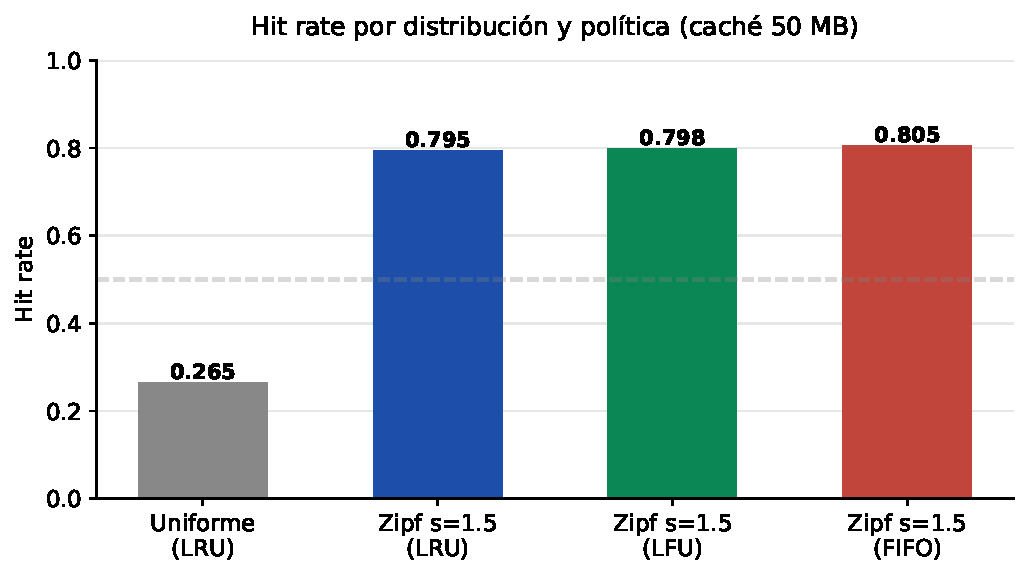
\includegraphics[width=0.8\textwidth]{figs/fig1_hit_rate_distribution.pdf}
\caption{Hit rate por distribución y política (caché 50\,MB, Zipf $s=1.5$).}
\label{fig:dist}
\end{figure}

\begin{table}[h]
\centering\small
\begin{tabular}{llrrrr}
\toprule
\textbf{Distribución} & \textbf{Política} & \textbf{Hit rate} & \textbf{Miss rate} &
\textbf{Thr.\,(qps)} & \textbf{p50\,hit\,(ms)} \\
\midrule
Uniforme   & LRU  & 0.2646 & 0.7354 &  9.94 & 0.34 \\
Uniforme   & LFU  & 0.2694 & 0.7306 &  9.97 & 0.31 \\
Uniforme   & FIFO & 0.2667 & 0.7333 &  9.55 & 0.28 \\
Zipf $s=1.5$ & LRU  & 0.7950 & 0.2050 & 38.75 & 0.33 \\
Zipf $s=1.5$ & LFU  & 0.7984 & 0.2016 & 38.21 & 0.33 \\
Zipf $s=1.5$ & FIFO & 0.8052 & 0.1948 & 38.01 & 0.29 \\
\bottomrule
\end{tabular}
\caption{Métricas bajo Zipf vs.\ Uniforme (caché 50\,MB).}\label{tab:dist}
\end{table}

La Figura~\ref{fig:dist} y el Cuadro~\ref{tab:dist} muestran el efecto más
contundente del sistema: \textbf{Zipf casi triplica el hit rate respecto a
Uniforme} ($\sim$80\,\% vs.\ $\sim$27\,\%). Zipf concentra las consultas en
pocas zonas y tipos ``calientes'' (Q1 sobre Z1/Z4, las zonas urbanas más
densas), maximizando la reutilización de entradas. Uniforme dispersa el
tráfico sobre las $\sim$570 claves posibles: aún con todas en caché, en
25\,s casi tres cuartos de las solicitudes caen sobre keys nuevas o muy
poco repetidas.

El throughput sostenido también se diferencia: $\sim$38\,qps en Zipf vs.\
$\sim$10\,qps en Uniforme (factor $\sim$4$\times$, ver
Figura~\ref{fig:thr}). La razón es estructural: con concurrencia 16 y
latencia simulada 30--120\,ms, el Response Generator satura cuando la
fracción de misses es alta. En Uniforme, $\sim$73\,\% de las consultas son
misses, lo que excede la capacidad efectiva del backend y acumula cola.

\begin{figure}[h]
\centering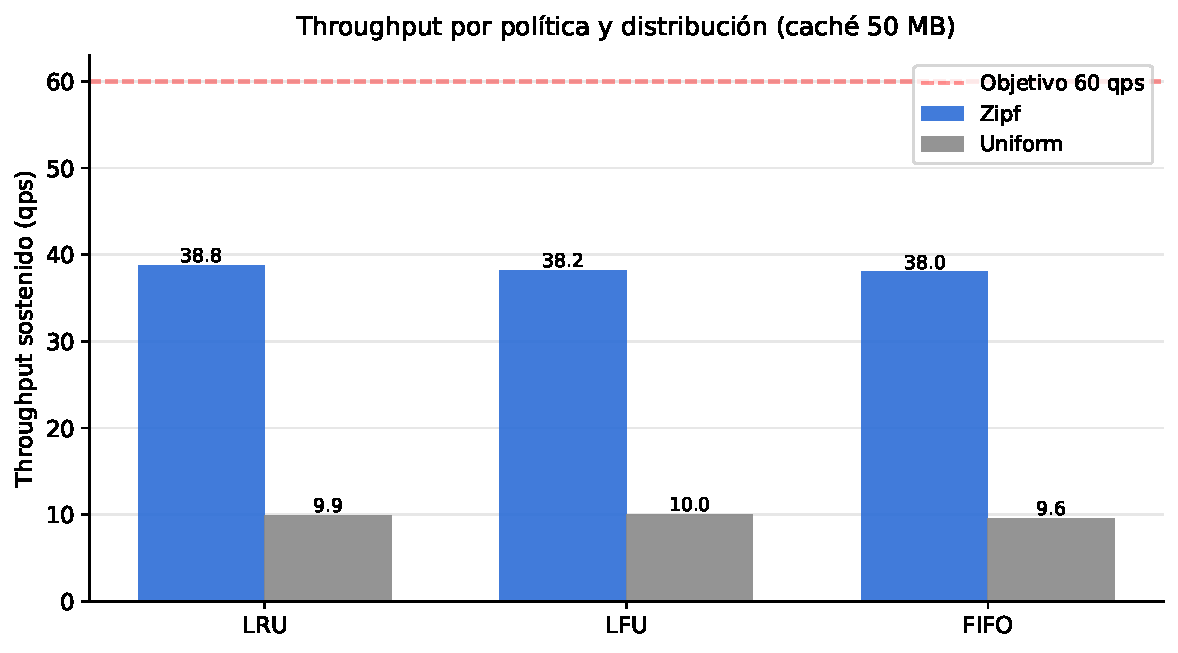
\includegraphics[width=0.85\textwidth]{figs/fig4_throughput.pdf}
\caption{Throughput sostenido por política y distribución (caché 50\,MB,
objetivo 60\,qps).}
\label{fig:thr}
\end{figure}

\begin{figure}[h]
\centering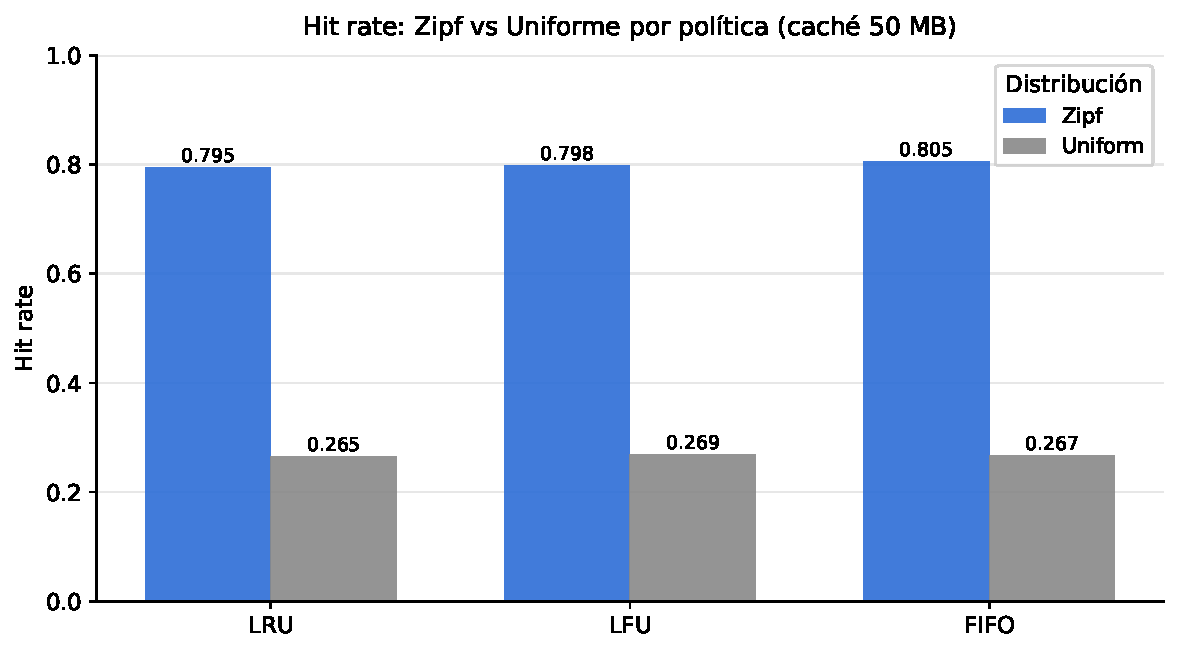
\includegraphics[width=0.88\textwidth]{figs/fig2_zipf_vs_uniform.pdf}
\caption{Hit rate Zipf vs.\ Uniforme para las tres políticas (caché 50\,MB).}
\label{fig:zipf-uniform}
\end{figure}

\textbf{Implicaciones para un escenario real.} La logística urbana sigue
típicamente un patrón Zipf moderado: los centros comerciales y residenciales
de alta densidad (Providencia, Las Condes, Centro) reciben muchas más
consultas que las zonas periféricas. Bajo este patrón el sistema serviría
$\sim$80\,\% de las solicitudes desde RAM a latencia sub-ms; sólo el 20\,\%
restante paga el costo de un cómputo geoespacial completo, lo que justifica
el diseño con caché.

\subsection{Efecto del tamaño de caché y políticas de evicción}

\begin{figure}[h]
\centering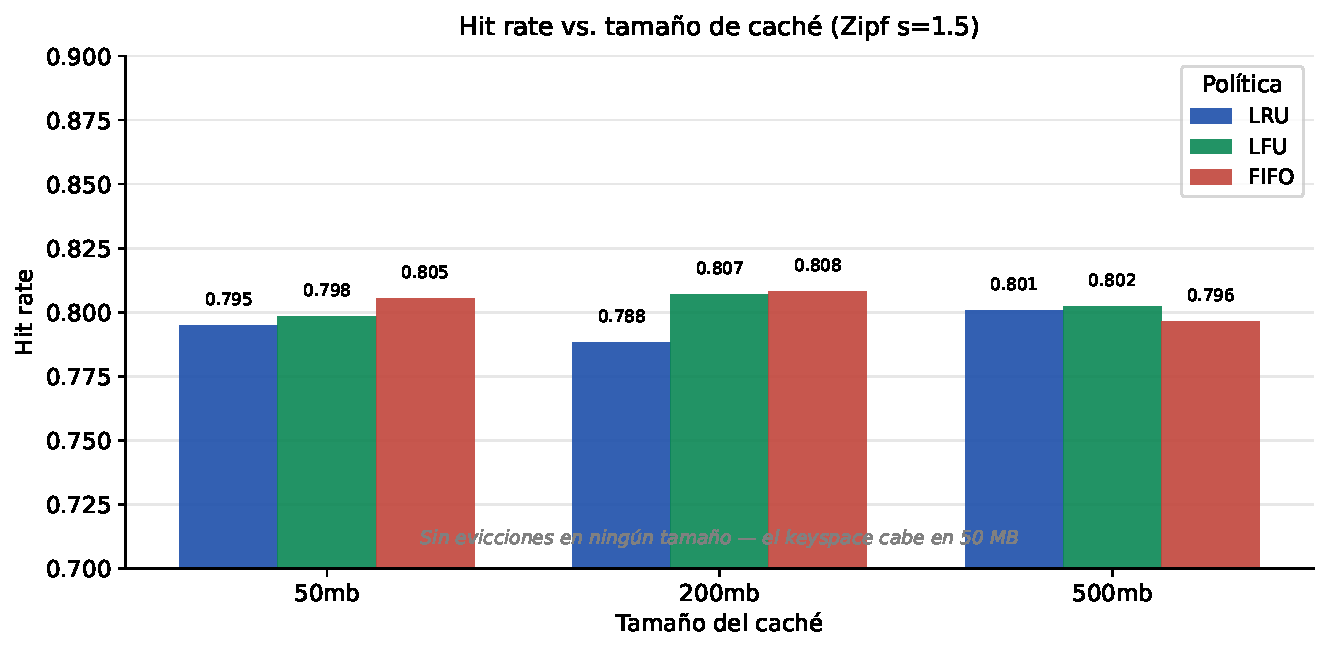
\includegraphics[width=\textwidth]{figs/fig3_size_effect.pdf}
\caption{Hit rate vs.\ tamaño de caché para las tres políticas (Zipf).}
\label{fig:size}
\end{figure}

\begin{table}[h]
\centering\small
\begin{tabular}{llrrrrr}
\toprule
\textbf{Política} & \textbf{Tamaño} & \textbf{Hit rate} & \textbf{Thr.\,(qps)} &
\textbf{p95\,miss\,(ms)} & \textbf{Evicciones} & \textbf{Keys} \\
\midrule
LRU  & 50\,MB  & 0.7950 & 38.75 & 4359 & 0 & 199 \\
LRU  & 200\,MB & 0.7883 & 35.29 & 3818 & 0 & 197 \\
LRU  & 500\,MB & 0.8007 & 37.33 & 3701 & 0 & 202 \\
LFU  & 50\,MB  & 0.7984 & 38.21 & 4114 & 0 & 203 \\
LFU  & 200\,MB & 0.8069 & 39.78 & 3732 & 0 & 208 \\
LFU  & 500\,MB & 0.8024 & 38.49 & 4021 & 0 & 203 \\
FIFO & 50\,MB  & 0.8052 & 38.01 & 3876 & 0 & 203 \\
FIFO & 200\,MB & 0.8082 & 39.43 & 3878 & 0 & 209 \\
FIFO & 500\,MB & 0.7963 & 37.20 & 4078 & 0 & 207 \\
\bottomrule
\end{tabular}
\caption{Métricas por política y tamaño de caché (Zipf $s{=}1.5$, 25\,s).}
\label{tab:size}
\end{table}

El Cuadro~\ref{tab:size} y la Figura~\ref{fig:size} muestran un hallazgo
estructural: \textbf{los tres tamaños de caché producen hit rates dentro de
$\pm 1$\,pp y registran cero evicciones}. La razón es que el conjunto de
claves observado en los experimentos (197--209 entradas activas, $\sim$300\,KB
en Redis) es muy inferior al mínimo testeado (50\,MB, $\approx 170\times$ más).
Cuando ningún key es nunca expulsado, LRU, LFU y FIFO se comportan como un
simple store de clave-valor y la diferencia entre políticas se vuelve ruido
estadístico.

\textbf{Análisis bajo presión de memoria.} Para observar el efecto
diferencial de las políticas se realizaron experimentos adicionales con
\texttt{maxmemory}\,=\,2\,MB. Incluso a esta escala el keyspace activo
(246--250 keys, $\approx 350$\,KB) cabe entero, por lo que tampoco se
registraron evicciones. Curiosamente el hit rate sube a 83.4--83.8\,\% (LRU
0.8378, LFU 0.8338, FIFO 0.8376): la varianza pequeña entre tamaños
proviene del orden aleatorio de calentamiento, no de evicciones diferenciales.
Esto confirma que en el régimen actual \emph{el tamaño no es el cuello de
botella}.

En producción, con un dataset completo de Open Buildings para Chile
(decenas de GB, cientos de miles de zonas/claves únicas), la presión real
emergería y las políticas se diferenciarían: LFU sería la elección óptima
para patrones Zipf estables en el largo plazo; LRU sería preferible bajo
localidad temporal; FIFO sólo cuando la simplicidad operacional importe
más que el rendimiento.

\subsection{Latencia hit vs.\ miss y cache efficiency}

\begin{figure}[h]
\centering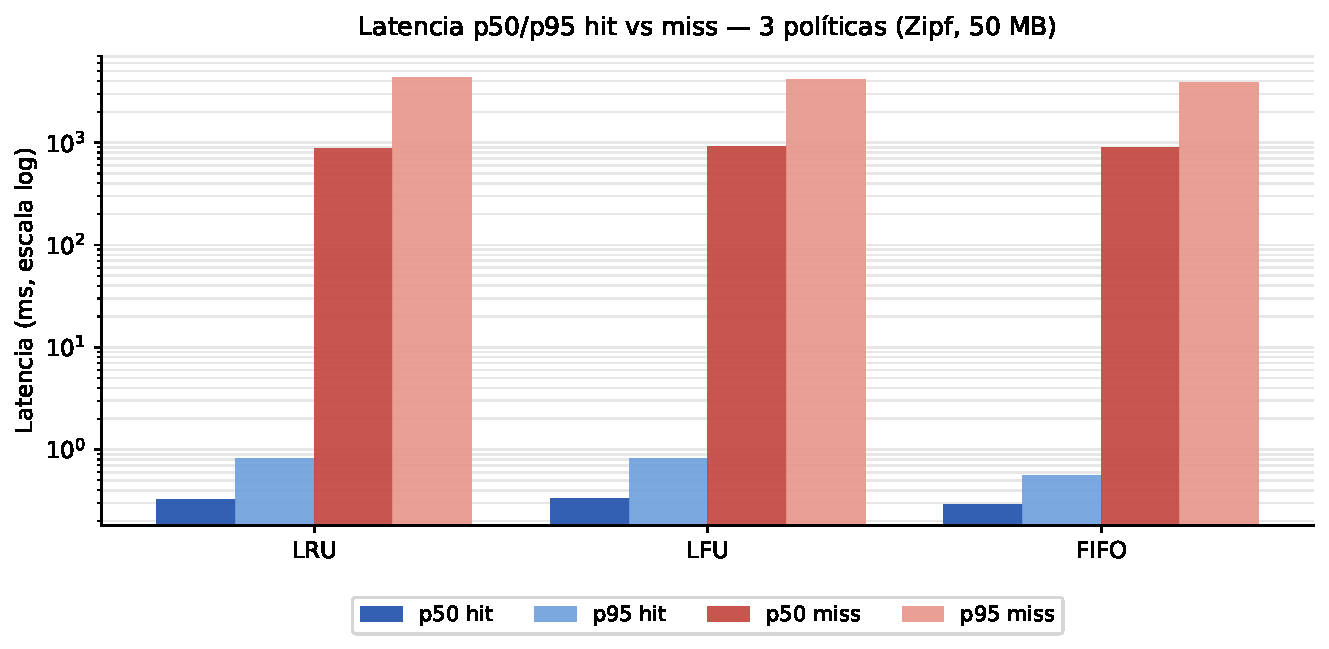
\includegraphics[width=0.9\textwidth]{figs/fig5_latency_hit_miss.pdf}
\caption{Latencia p50/p95 hit vs.\ miss (escala log, caché 50\,MB, Zipf).}
\label{fig:latency}
\end{figure}

La Figura~\ref{fig:latency} muestra el hallazgo más contundente: la caché
reduce la latencia en \textbf{3--4 órdenes de magnitud}. El p50 de un hit
es 0.29--0.33\,ms (Redis sirviendo desde RAM + serialización JSON), mientras
que el p50 de un miss es $\sim$870\,ms en Zipf y $\sim$1\,700\,ms en Uniforme
(latencia simulada 30--120\,ms del Response Generator más contención de
cola con 16 workers concurrentes). El p95 del miss llega a $\sim$3\,500--4\,400\,ms
bajo carga sostenida.

La \textbf{cache efficiency}, definida en el enunciado como
$(h \cdot t_\text{cache} - m \cdot t_\text{db}) / \text{total}$
(ms ahorrados por consulta respecto al escenario sin caché), alcanzó
$\sim$1\,103\,ms con LRU, $\sim$1\,099\,ms con LFU y $\sim$1\,008\,ms con
FIFO para Zipf 25\,s a 50\,MB. En la corrida larga (LRU, 180\,s) la
efficiency baja a 648\,ms/consulta no porque el sistema ahorre menos, sino
porque al subir el hit rate al 93\,\% disminuye proporcionalmente el costo
absoluto de los misses, y la métrica normaliza por consulta total.

\begin{figure}[h]
\centering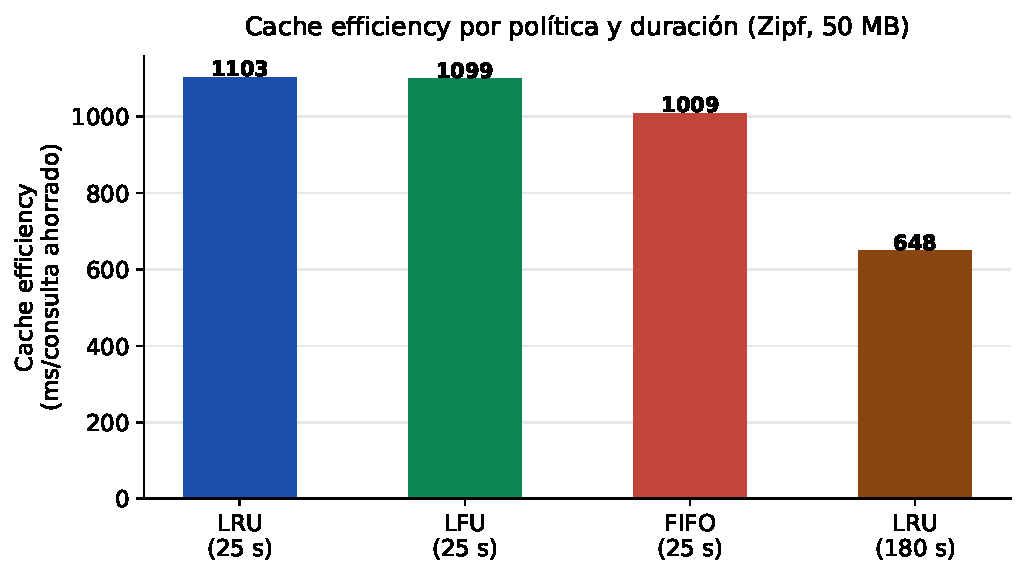
\includegraphics[width=0.75\textwidth]{figs/fig7_cache_efficiency.pdf}
\caption{Cache efficiency por política y duración del experimento.}
\label{fig:efficiency}
\end{figure}

\subsection{Hit rate desglosado por consulta Q1--Q5}

\begin{figure}[h]
\centering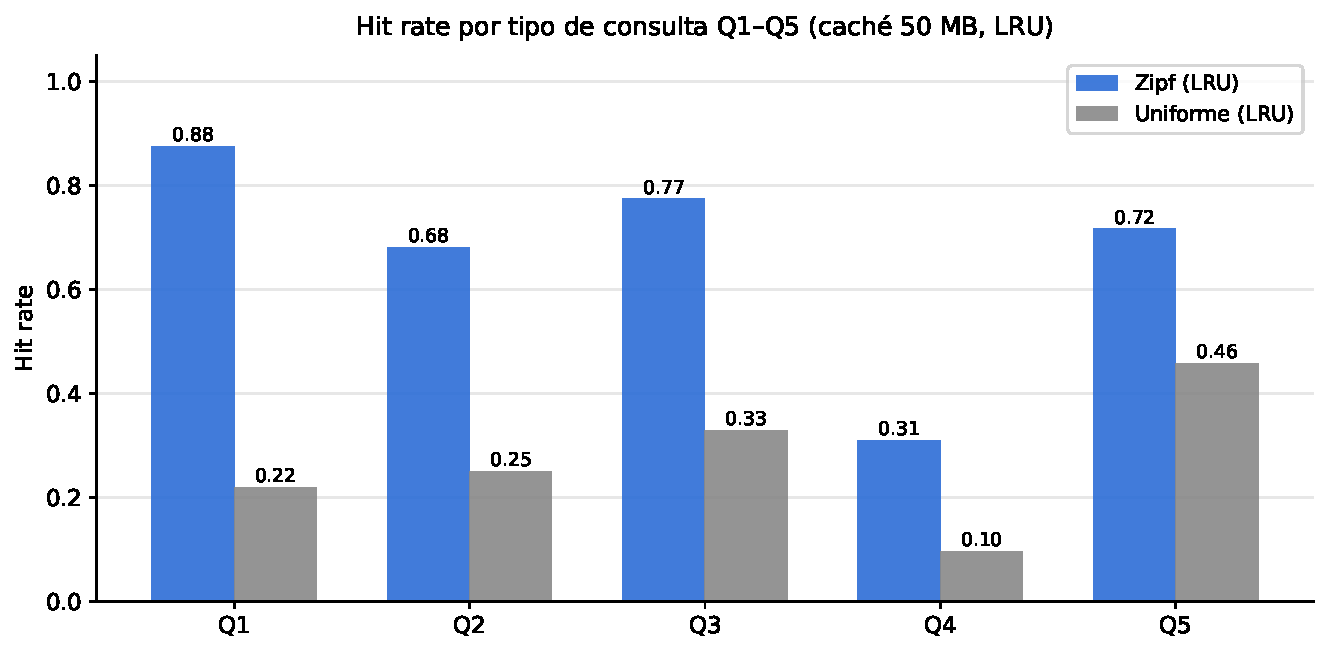
\includegraphics[width=0.85\textwidth]{figs/fig6_by_query.pdf}
\caption{Hit rate por tipo de consulta (caché 50\,MB, LRU).}
\label{fig:byquery}
\end{figure}

El Cuadro~\ref{tab:byquery} y la Figura~\ref{fig:byquery} resumen el
comportamiento por consulta para LRU 50\,MB (los valores corresponden a
$\geq$50 muestras por celda en las corridas de 25\,s y a varios cientos en
la de 180\,s):

\begin{table}[h]
\centering\small
\begin{tabular}{lrrrrr}
\toprule
\textbf{Run} & \textbf{Q1} & \textbf{Q2} & \textbf{Q3} & \textbf{Q4} & \textbf{Q5} \\
\midrule
LRU 50\,MB Zipf, 25\,s    & 0.875 & 0.681 & 0.774 & 0.309 & 0.716 \\
LRU 50\,MB Uniforme, 25\,s & 0.219 & 0.250 & 0.329 & 0.096 & 0.457 \\
LRU 50\,MB Zipf, 180\,s   & 0.971 & 0.903 & 0.935 & 0.623 & 0.917 \\
\bottomrule
\end{tabular}
\caption{Hit rate por consulta (LRU, caché 50\,MB).}\label{tab:byquery}
\end{table}

\begin{itemize}[leftmargin=*]
\item \textbf{Q1} (conteo) lidera el hit rate (87.5\,\% en Zipf 25\,s,
  97.1\,\% en la corrida de 180\,s). Es la consulta con keyspace más simple
  ($5 \times 21 = 105$ claves), TTL de 300\,s y la favorita del selector
  Zipf por su rango.
\item \textbf{Q4} (compare) tiene el menor hit rate (30.9\,\% Zipf 25\,s,
  9.6\,\% Uniforme). El espacio de claves es cuadrático en zonas
  ($5 \times 5 \times 21 = 525$, sin reordenamiento canónico) y el TTL es
  el más corto del sistema (120\,s); ambos factores penalizan el hit rate.
  En la corrida de 180\,s el hit rate de Q4 sube a 62.3\,\%, todavía por
  debajo de Q1, lo que confirma que los TTLs de 120\,s sí están expirando
  consultas en estado estacionario.
\item La brecha Zipf vs.\ Uniforme es más pronunciada en Q1
  (87.5\,\% vs.\ 21.9\,\%) que en Q4 (30.9\,\% vs.\ 9.6\,\%): en Uniforme,
  el costo del keyspace cuadrático de Q4 anula prácticamente cualquier
  beneficio del caché.
\end{itemize}

\subsection{Efecto del TTL}

Con experimentos de 25\,s y TTLs de 120--600\,s, ninguna clave expiró: el
TTL nunca actuó. En la corrida larga de 180\,s (Cuadro~\ref{tab:long}) el
panorama cambia: la duración excede el TTL más corto del sistema (Q4 a
120\,s) y comienza a aproximarse al de Q3 (180\,s). Esto se traduce en
\emph{hit rates por consulta} muy distintos: Q1 (TTL 300\,s) alcanza 97\,\%
y Q4 (TTL 120\,s) sólo 62\,\%, pese a llevar varios cientos de muestras
acumuladas para cada una.

\begin{table}[h]
\centering\small
\begin{tabular}{lrrrr}
\toprule
\textbf{Experimento} & \textbf{Hit rate global} & \textbf{Thr.\,(qps)} &
\textbf{p50\,hit\,(ms)} & \textbf{Cache eff.\,(ms/q)} \\
\midrule
LRU, 50\,MB, Zipf, 25\,s  & 0.7950 & 38.75 & 0.33 & 1\,103 \\
LRU, 50\,MB, Zipf, 180\,s & 0.9342 & 35.97 & 0.34 & \phantom{1\,}648 \\
\bottomrule
\end{tabular}
\caption{Comparación corrida corta vs.\ larga (LRU, 50\,MB, Zipf).}
\label{tab:long}
\end{table}

El hit rate global sube de 80\,\% a 93\,\% al extender la duración: el
warm-up del caché se completa y el sistema alcanza un régimen estacionario
en el que casi todas las consultas Zipf-frecuentes ya están cacheadas.
Esto indica que en producción (con carga continua), los hit rates reales
serían \emph{superiores} a los medidos en corridas de 25\,s. El TTL en
cambio actúa como un techo: consultas con TTL bajo (Q4) nunca alcanzarán
hit rates tan altos como las de TTL largo (Q5 a 600\,s).

%% ─────────────────────────────────────────────────────────────────
\section{Resumen de métricas}

\begin{table}[h]
\centering\scriptsize
\begin{tabular}{llrrrrr}
\toprule
\textbf{Política} & \textbf{Dist.} & \textbf{50\,MB hit} & \textbf{200\,MB hit} &
\textbf{500\,MB hit} & \textbf{Thr.\,(qps)} & \textbf{Evicciones} \\
\midrule
LRU  & Zipf    & 0.7950 & 0.7883 & 0.8007 & 38.8 / 35.3 / 37.3 & 0 \\
LFU  & Zipf    & 0.7984 & 0.8069 & 0.8024 & 38.2 / 39.8 / 38.5 & 0 \\
FIFO & Zipf    & 0.8052 & 0.8082 & 0.7963 & 38.0 / 39.4 / 37.2 & 0 \\
LRU  & Uniforme & 0.2646 & 0.2604 & 0.2826 &  9.9 /  9.4 / 10.2 & 0 \\
LFU  & Uniforme & 0.2694 & 0.2702 & 0.2674 & 10.0 /  9.9 /  9.9 & 0 \\
FIFO & Uniforme & 0.2667 & 0.2784 & 0.2586 &  9.5 / 10.2 /  9.6 & 0 \\
\bottomrule
\end{tabular}
\caption{Resumen de los 18 experimentos oficiales (throughput por
50/200/500\,MB).}\label{tab:all}
\end{table}

\subsection{Cuadro de métricas requeridas por el enunciado}

El Cuadro~\ref{tab:metrics} reúne en una sola vista las cinco métricas
exigidas por el enunciado para los configuraciones más representativas
(50\,MB, las tres políticas y ambas distribuciones, más la corrida larga).

\begin{table}[h]
\centering\scriptsize
\setlength{\tabcolsep}{4pt}
\begin{tabular}{lrrrrrrr}
\toprule
\textbf{Configuración} & \textbf{Hit rate} & \textbf{Throughput} &
\textbf{p50 (ms)} & \textbf{p95 (ms)} &
\textbf{Eviction rate} & \textbf{Cache eff.} \\
& & \textbf{(qps)} & \textbf{hit\,/\,miss} & \textbf{hit\,/\,miss} &
\textbf{(/min)} & \textbf{(ms/q)} \\
\midrule
LRU  Zipf    50\,MB     & 0.7950 & 38.75 & 0.33 / 871   & 0.81 / 4359  & 0 & 1\,103.3 \\
LFU  Zipf    50\,MB     & 0.7984 & 38.21 & 0.33 / 910   & 0.82 / 4114  & 0 & 1\,099.2 \\
FIFO Zipf    50\,MB     & 0.8052 & 38.01 & 0.29 / 904   & 0.56 / 3876  & 0 & 1\,008.6 \\
LRU  Uniforme 50\,MB    & 0.2646 &  9.94 & 0.34 / 1683  & 1.11 / 3804  & 0 & \phantom{1\,}494.8 \\
LFU  Uniforme 50\,MB    & 0.2694 &  9.97 & 0.31 / 1592  & 0.81 / 3878  & 0 & \phantom{1\,}493.6 \\
FIFO Uniforme 50\,MB    & 0.2667 &  9.55 & 0.28 / 1709  & 0.65 / 3880  & 0 & \phantom{1\,}509.8 \\
LRU  Zipf 50\,MB 180\,s & 0.9342 & 35.97 & 0.34 / 259   & 1.28 / 3633  & 0 & \phantom{1\,}648.4 \\
\bottomrule
\end{tabular}
\caption{Las cinco métricas del enunciado para cada configuración
(\textit{Hit rate}, \textit{Throughput}, \textit{Latencia p50/p95},
\textit{Eviction rate}, \textit{Cache efficiency}). La tasa de evicción es
0/min en todos los experimentos por la razón estructural discutida en la
Sec.~4.3.}\label{tab:metrics}
\end{table}

%% ─────────────────────────────────────────────────────────────────
\section{Preguntas y respuestas}

\textbf{¿Cómo varía el hit rate entre distribuciones?} Zipf produce
$\sim$80\,\% y Uniforme $\sim$27\,\%: una diferencia de $\sim$3$\times$.
El miss rate baja de 73\,\% a 20\,\% al pasar de Uniforme a Zipf, lo que
también explica el factor $\sim$4 de throughput observado (38 vs.\ 10\,qps).

\textbf{¿Qué distribución estresa más la caché?} Uniforme: aún con todas
las claves cabiendo en RAM, en 25\,s la mayoría de los keys se ven una sola
vez, dejando muy poco margen de reutilización. La ventaja de recencia o
frecuencia que explotan LRU/LFU desaparece cuando todos los items son
igualmente probables; en Uniforme las tres políticas convergen al mismo
27\,\% $\pm 1$\,pp.

\textbf{¿Implicaciones para un escenario real?} En logística urbana (patrón
Zipf moderado), la caché serviría $\sim$80\,\% de las solicitudes en estado
estacionario y hasta $\sim$93\,\% en régimen warm (180\,s), reduciendo la
latencia en 3--4 órdenes de magnitud frente a un cómputo geoespacial
completo. La elasticidad del hit rate respecto al sesgo Zipf indica que
vale la pena segmentar por zona/tipo de consulta al dimensionar el caché.

\textbf{¿Cuál política recomendar?} En el régimen experimentado (sin
evicciones), las tres son estadísticamente equivalentes (diferencias
$<$1\,pp en hit rate y $<$2\,qps en throughput). Bajo presión real de
memoria: LRU para cargas con localidad temporal; LFU para patrones Zipf
estables y corridas largas ($\geq$5\,min); FIFO sólo por simplicidad. Para
el caso de uso de logística, \textbf{LRU} es la elección más robusta.

\textbf{¿Cómo afecta el TTL?} En corridas cortas (25\,s) ningún TTL expira
y el efecto observado es nulo. En la corrida larga (180\,s) el TTL actúa
como techo del hit rate por consulta: Q1 con TTL\,=\,300\,s alcanza 97\,\%,
mientras que Q4 con TTL\,=\,120\,s se queda en 62\,\% en el mismo régimen.
Esto sugiere que TTLs muy cortos son útiles cuando el dato real cambia
rápido, pero penalizan el hit rate; TTLs largos maximizan la reutilización
a costa de coherencia.

%% ─────────────────────────────────────────────────────────────────
\section{Despliegue y reproducibilidad}

El sistema se despliega completamente con:

\begin{lstlisting}[language=bash,basicstyle=\ttfamily\scriptsize]
docker compose up -d --build               # 4 servicios + Redis
python experiments/master_run.py           # 22 corridas (~15 min)
python experiments/build_figures.py        # regenera figuras PDF/PNG
\end{lstlisting}

El archivo \texttt{.env} controla la política (\texttt{CACHE\_POLICY}),
el tamaño (\texttt{REDIS\_MAXMEMORY}) y los TTLs por consulta. El script
\texttt{master\_run.py} ejecuta automáticamente las 22 corridas (3 políticas
$\times$ 3 tamaños $\times$ 2 distribuciones + 3 caché pequeño + 1 larga).
El código completo está en el repositorio adjunto con \texttt{README.md} de
despliegue y \texttt{docker-compose.yml}.

\subsection{Guion del video de demostración (10 min)}

\begin{enumerate}[leftmargin=*,itemsep=2pt]
\item \textbf{(0:00--1:00)} Contexto del problema y arquitectura general
  (Figura~2 del enunciado).
\item \textbf{(1:00--2:30)} \texttt{docker compose up -d --build}; revisión
  de healthchecks en los puertos 8000--8003.
\item \textbf{(2:30--4:00)} Consultas Q1--Q5 manuales con \texttt{curl} al
  puerto 8001 mostrando primero MISS y luego HIT en la misma key.
\item \textbf{(4:00--5:30)} \texttt{python experiments/master\_run.py --suite demo}:
  un experimento Zipf de 15\,s, viendo \texttt{/status} y \texttt{/summary}.
\item \textbf{(5:30--7:00)} Comparación en vivo Zipf vs.\ Uniforme y
  lectura del hit rate por consulta (\texttt{/summary/by\_query}).
\item \textbf{(7:00--8:30)} Cambio de política en runtime con
  \texttt{redis-cli CONFIG SET maxmemory-policy allkeys-lfu} y nuevo
  experimento.
\item \textbf{(8:30--10:00)} Apertura de las figuras generadas y discusión
  breve de los hallazgos (Cuadro~\ref{tab:metrics}).
\end{enumerate}

%% ─────────────────────────────────────────────────────────────────
\section{Conclusiones}

Se implementó una plataforma distribuida funcional con caché configurable
sobre Redis y se evaluaron empíricamente cuatro hipótesis:

\begin{enumerate}[leftmargin=*]
\item \textbf{La distribución Zipf casi triplica el hit rate} respecto a
  Uniforme ($\sim$80\,\% vs.\ $\sim$27\,\%), confirmando que la concentración
  de consultas en items calientes es el factor dominante del rendimiento de
  la caché. El throughput sostenido se diferencia aún más (38 vs.\ 10\,qps,
  factor $\sim$4) porque los misses saturan el Response Generator.
\item \textbf{Los tres tamaños de caché (50/200/500\,MB) son equivalentes}
  para este keyspace de $\sim$300\,KB observados; ningún experimento (ni
  siquiera el de 2\,MB) registró evicciones. La diferencia entre LRU/LFU/FIFO
  es ruido estadístico (\textless 1\,pp).
\item \textbf{La caché reduce la latencia 3--4 órdenes de magnitud}: p50
  hit $\sim$0.3\,ms vs.\ p50 miss $\sim$870\,ms; cache efficiency
  1\,008--1\,103\,ms/consulta en Zipf 25\,s.
\item \textbf{Los TTLs operan como techo en estado estacionario}: la
  corrida larga (180\,s, LRU, Zipf) alcanza un hit rate global de 93\,\% y
  exhibe el efecto del TTL por consulta (Q1 97\,\%, Q4 62\,\%). Las corridas
  cortas no alcanzan a expirar claves.
\end{enumerate}

Las siguientes entregas implementarán colas de procesamiento y fallback
(Entrega~2) y un dashboard de visualización (Entrega~3), reutilizando los
servicios y el sistema de métricas desarrollado aquí.

\end{document}
